Dit hoofdstuk behandelt de werking van onze software waarmee we onze hardware aansturen. We bespreken op welke manier we met de Arduino de IR-sensoren inlezen en aan de hand hiervan bijsturen, hoe we de snelheid meten, hoe RFID-tags ingelezen worden en hoe de Bluetooth-communicatie met de Raspberry Pi werkt.

\section{IR-sensoren inlezen}
Voor het inlezen van de sensoren wordt gebruik gemaakt van \'e\'en analoge pin, met deze pin lezen we de waardes van alle acht sensoren in via een multiplexer. Deze multiplexer wordt aangestuurd aan de hand van drie digitale pinnen die dienst doen als bit select. Om de tijdsduur voor het inlezen van de infrarood-sensoren via de multiplexer te minimaliseren lezen we deze in aan de hand van Gray-code. De volgorde van inlezen wordt verduidelijkt in tabel~\vref{table:graycode}. De ingelezen waarden worden opgeslagen in een array van acht integers. De waardes in de array worden vervolgens gedigitaliseerd aan de hand van een grenswaarde, hiervoor hebben we de waarde $300$ gekozen. Indien de sensorwaarde onder deze grens ligt ziet de sensor een witte ondergrond en krijgt dit digitaal een waarde '$1$', als de waarde boven de grens ligt komt dit overeen met een zwarte ondergrond en een digitale waarde '$0$'. 

\begin{table}[H]
	\centering
	\begin{tabular}{|l|l|l|l|l|l|}
		\hline
		\# & Bit Select 2 & Bit Select 1 & Bit Select 0 & MUX-pin & Sensor      \\ \hline
		0  & 0            & 0            & 0            & 13      & Vooraan 2   \\ \hline
		1  & 0            & 0            & 1            & 14      & Vooraan 3   \\ \hline
		3  & 0            & 1            & 1            & 12      & Vooraan 1   \\ \hline
		2  & 0            & 1            & 0            & 15      & Vooraan 4   \\ \hline
		6  & 1            & 1            & 0            & 2       & Achteraan 3 \\ \hline
		7  & 1            & 1            & 1            & 7       & Achteraan 2 \\ \hline
		5  & 1            & 0            & 1            & 5       & Achteraan 1 \\ \hline
		4  & 1            & 0            & 0            & 7       & Achteraan 4 \\ \hline
	\end{tabular}
	\caption{Inlezen van sensoren aan de hand van Grey-code}
	\label{table:graycode}
\end{table}

\section{Rijden en PID-regeling}
\subsection{Bijsturen van de motoren}
De snelheid van de motoren wordt geregeld aan de hand van Pulse Width Modulation. Softwarematig gebeurt dit met 8 bits en kunnen we de snelheid dus schalen tussen 0 en 255. Voor het nemen van een bocht maken we gebruik van een factor $F$ die we schalen tussen $-100$ en $100$. Deze factor drukt uit hoeveel \% \'e\'en van de wielen moet vertragen. Indien $F=-100$ bedraagt zal het wagentje volledig links draaien aangezien het linkerwiel niet meer aangestuurd wordt. Omgekeerd draait het wagentje volledig naar rechts als $F = 100$. Bij $F=0$ blijven beide wielen aan dezelfde constante snelheid draaien.
\subsection{Berekening van foutwaarde}
Nu de sensoren ingelezen kunnen worden is het mogelijk om aan de hand hiervan de positie van het wagentje ten opzichte van de zijlijn te bepalen.
Hiermee kan vervolgens het wagentje correct bijgestuurd worden om deze lijn te volgen. Om dit te realiseren wordt PID-regeling toegepast.
Deze PID-regeling gebeurt aan de hand van een foutwaarde die afgeleid wordt uit de ingelezen sensorwaarden, aan elke sensor wordt dus een gewicht toegekend die een maat geeft voor de afwijking ten opzichte van de witte lijn. Deze gewichten vindt u in tabel~\vref{table:sensorgewicht}.

\begin{table}[H]
	\centering
	\begin{tabular}{lllll}
		\hline
		\multicolumn{1}{|l|}{}           & \multicolumn{1}{l|}{Vooraan 1}   & \multicolumn{1}{l|}{Vooraan 2}   & \multicolumn{1}{l|}{Vooraan 3}   & \multicolumn{1}{l|}{Vooraan 4}   \\ \hline
		\multicolumn{1}{|l|}{Foutwaarde} & \multicolumn{1}{l|}{-3}          & \multicolumn{1}{l|}{-1}          & \multicolumn{1}{l|}{1}           & \multicolumn{1}{l|}{3}           \\ \hline
		&                                  &                                  &                                  &                                  \\ \hline
		\multicolumn{1}{|l|}{}           & \multicolumn{1}{l|}{Achteraan 1} & \multicolumn{1}{l|}{Achteraan 2} & \multicolumn{1}{l|}{Achteraan 3} & \multicolumn{1}{l|}{Achteraan 4} \\ \hline
		\multicolumn{1}{|l|}{Foutwaarde} & \multicolumn{1}{l|}{3}           & \multicolumn{1}{l|}{1}           & \multicolumn{1}{l|}{-1}          & \multicolumn{1}{l|}{-3}           \\ \hline
	\end{tabular}
	\caption{Gewichten van sensoren}
	\label{table:sensorgewicht}
\end{table}

De foutwaarde van de voorste sensoren wordt nu berekend met volgende formule:
\begin{gather*}
E_{vooraan} = \frac{\sum\limits_{i=1}^{4}S_{vooraan,i}\cdot G_{vooraan,i}}{\sum\limits_{i=1}^{4}S_{vooraan,i}}
\end{gather*}
Analoog wordt de foutwaarde voor de achterste sensoren gegeven door:
\begin{gather*}
E_{achteraan} = \frac{\sum\limits_{i=1}^{4}S_{achteraan,i}\cdot G_{achteraan,i}}{\sum\limits_{i=1}^{4}S_{achteraan,i}}\\
\end{gather*}
Hierin is $S_i$ de digitale waarde in de array, zoals reeds vermeld is deze gelijk aan $1$ indien sensor $i$ een witte ondergrond ziet en $0$ wanneer de ondergrond zwart is. $G_i$ is het gewicht van de sensor in kwestie.\\
De totale foutwaarde $E_{totaal}$ wordt dan bepaald door beide foutwaarden op te tellen:
\begin{gather*}
E_{totaal}=E_{vooraan}+E_{achteraan}
\end{gather*}
Deze foutwaarde zal negatief zijn wanneer het wagentje teveel naar rechts afwijkt ten opzichte van de zijlijn, omgekeerd is deze fout positief als het wagentje te veel naar links rijdt. Als het wagentje perfect rechtdoor rijdt zullen de foutwaardes elkaar compenseren zodat de foutwaarde $0$ wordt. 
\subsection{PID-regeling}
Nu we een maat hebben voor de afwijking ten opzichte van de zijlijn kunnen we de PID-regeling toepassen. Hierbij wordt de factor tussen $-100$ en $100$ bepaald die we gebruiken voor het bijsturen van de motoren, deze factor wordt als volgt bepaald:
\begin{gather*}
	F = K_P \cdot E_P + K_I \cdot E_I + K_D \cdot E_D\\
\end{gather*}
Hierin is:
\begin{itemize}
	\item $F$ = factor voor het bijsturen van de motoren
	\item $E_P = E_{totaal}$ = proportionele term fout
	\item $E_I = \sum E_{totaal}$ = integrerende term fout
	\item $E_D = E_{totaal} - E_{totaal,vorig}$ = differenti\"erende term fout
	\item $K_P$ = constante waarde om de invloed van de proportionele term te schalen
	\item $K_I$ = constante waarde om de invloed van de integrerende term te schalen
	\item $K_D$ = constante waarde om de invloed van de differenti\"erende term te schalen
\end{itemize}
De constanten $K_P$,$K_I$ en $K_D$ bepalen in sterke mate de werking van de PID-regeling. Aangezien het afstellen van deze waarden praktisch gezien via een trial-and-error-proces verloopt worden deze waarden in de setup opgevraagd bij de Raspberry Pi Python Shell, hoe dit precies gebeurt wordt besproken in sectie~\vref{sec:bluetooth-communicatie-naar-raspberry-pi}. We merken dat we voor de meeste circuits de beste resultaten halen met $K_P=12$, $K_I=1$ en $K_D=25$\\

In het geval dat de voorste sensorarray teveel van de baan afwijkt wordt afgestapt van werkelijke PID-regeling en wordt er overgeschakeld naar een soort pseudo PID-regeling waarbij de foutwaarde aan de hand van de laatst bepaalde foutwaarde steeds ge\"incrementeerd wordt. Wanneer de voorste sensorarray zich opnieuw boven de lijn bevindt hervat de normale PID-regeling terug.


\section{Snelheid meten}
In sectie~\vref{sec:hall-sensor} bespraken we reeds op welke manier we twee magneten bevestigden in de wielas die passeren bij een SS41 Hall-sensor.
Deze twee magneten zorgen door de tegengestelde polarisatie dat de output van de SS41 omschakelt van hoog ($5\,\mathrm{V}$) naar laag ($0\,\mathrm{V}$) en vice versa bij het passeren van \'e\'en van de magneten. 
Binnen een tijdsinterval $\Delta t$ tellen we het aantal keer $C$ dat deze omschakeling optreedt. Het aantal rotaties in dit interval is dan de helft van het aantal keer dat de sensoroutput omgeschakeld is. Wetende dat de diameter $D$ van het wiel $7\,\mathrm{cm}$ bedraagt kunnen we de snelheid $v$ als volgt berekenen:

\begin{gather*}
v=\frac{\Delta x}{\Delta t} = \frac{\frac{C}{2}\cdot\pi\cdot D}{\Delta t}
\end{gather*}
De snelheid van ons wagentje wordt voortdurend berekend over periodes van 10\,s. Daarna wordt deze ook verzonden over Bluetooth.

\section{RFID-tags inlezen}
De software voor het inlezen van de RFID-tags maakt gebruik van libraries die te vinden zijn op de GitHub-pagina van Elechouse\footnote{\url{https://github.com/elechouse/PN532}}. Aangezien het inlezen van een tag over I\textsuperscript{2}C enkele tientallen milliseconden kan duren wordt om de 100\,ms gepolled of een nieuwe tag aanwezig is, op deze manier wordt het inlezen van andere sensoren en bijsturen van de motoren in mindere mate onderbroken. Indien er een nieuwe tag aanwezig is zal de ID van deze tag uitgelezen en opgeslagen worden aan de hand van de Elechouse-library. Vervolgens worden deze gegevens via Bluetooth naar onze Raspberry Pi verzonden, deze communicatie wordt besproken in volgend hoofdstuk.

\section{Bluetooth-communicatie naar Raspberry Pi}\label{sec:bluetooth-communicatie-naar-raspberry-pi}
\subsection{Arduino met HC05-module als Slave}
De HC05-module laat ons toe om via Bluetooth informatie over ons wagentje te verzenden naar onze Raspberry Pi. We zullen deze module gebruiken als Slave en de verbinding maken vanaf onze Raspberry Pi. Aangezien deze module seri\"ele communicatie voorziet gebruiken we de SoftwareSerial-library van Arduino. We defini\"eren dus een Transmit- en Receive-pin en maken een SoftwareSerial-object aan waaraan we deze pinnen meegeven. In de setup starten we de seri\"ele Bluetooth-communicatie op met een baudrate van 9600 bits per seconde. Vervolgens kunnen we in de rest van ons programma eenvoudigweg data printen over Bluetooth met \emph{println}-instructies, of integers ontvangen over Bluetooth inlezen met \emph{parseInt()}.

\subsection{Raspberry Pi 3 met ingebouwde Bluetooth-adapter als Master}
Aan de kant van de Raspberry Pi 3, die we als Master gebruiken, dienen we eerst correct verbinding te maken met de HC05-Bluetooth-module. Daarvoor voeren we volgend script uit:
\lstinputlisting[captionpos=b,caption=Script om verbinding te maken met HC05-module,label=lst:bt]{robbiebt.sh}
Hierin is 98:D3:32:11:64:0C de hexadecimale voorstelling van het adres van onze Bluetooth-module. Eerst wordt verbinding gemaakt tussen de ingebouwde adapter van de RPi en de HC05. Vervolgens binden we deze verbinding aan rfcomm-poort 1 en monitoren we het verkeer op deze poort.\\
Het verzenden en lezen van data wordt nu gedaan aan de hand van een Python-script waarin we gebruik maken van de Python-library serial. Het script leest voortdurend data in die ontvangen wordt van de Arduino. Indien deze data de gemeten snelheid of de gegevens van ingelezen RFID-tags bevat wordt deze op het scherm van onze Raspberry Pi afgeprint. In de setup van de Arduino wordt een token verzonden naar de RPi, als deze token ontvangen wordt kunnen we in de Python Shell de snelheid en de PID-constanten waarmee het wagentje moet vertrekken meegeven. Op deze manier hoeven we niet steeds te herprogrammeren om deze waarden aan te passen. Een voorbeeld van het resultaat in de Python Shell ziet u in figuur~\vref{fig:bluetoothoutput}.

\begin{figure}[H]
	\centering
	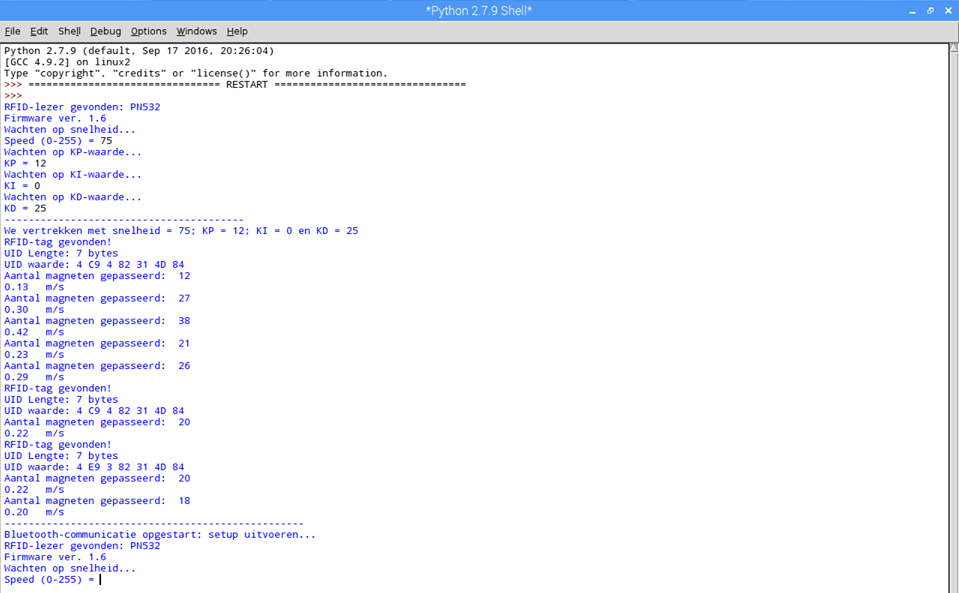
\includegraphics[width=\textwidth]{bluetoothoutputvoorbeeldbijgesneden.png}
	\caption{Voorbeeld van ingeven PID-constanten en ontvangen data in Python Shell\label{fig:bluetoothoutput}}
\end{figure}

\section{Custom board progammeren}
